%=========== ΛΥΣΗ - ΘΕΜΑ Β_19 ===========
\begin{thema}{Β}
Δίνεται η συνάρτηση $f(x) = ax^3 - 3x + \beta$, όπου $a, \beta \in \mathbb{R}$. Η γραφική παράσταση της $f$ διέρχεται από το σημείο $A(0,1)$ και η $f$ παρουσιάζει τοπικό ακρότατο στο $x_0 = 1$.

\begin{erwthma}

% -------------------------------------------------------
% α) Εύρεση a και β
% -------------------------------------------------------
\item Αφού η $C_f$ διέρχεται από το $A(0,1)$, ισχύει $f(0) = 1$:
\[
f(0) = a\cdot0 - 3\cdot0 + \beta = \beta = 1.
\]
Επομένως $\beta = 1$.

Αφού η $f$ παρουσιάζει τοπικό ακρότατο στο $x_0 = 1$ και είναι παραγωγίσιμη εκεί, από το Θεώρημα Fermat ισχύει $f'(1) = 0$:
\[
f'(x) = 3ax^2 - 3 \Rightarrow f'(1) = 3a - 3 = 0 \Rightarrow a = 1.
\]
Επομένως $a = 1$ και $\beta = 1$, άρα $f(x) = x^3 - 3x + 1$.

% -------------------------------------------------------
% β) Μονοτονία και κυρτότητα
% -------------------------------------------------------
\item \textbf{Μονοτονία.}
\[
f'(x) = 3x^2 - 3 = 3(x^2 - 1) = 3(x-1)(x+1).
\]
Βρίσκουμε ρίζες και πρόσημο της $f'$:
\begin{itemize}
    \item $f'(x) = 0 \Leftrightarrow x = \pm 1$
    \item $f'(x) > 0 \Leftrightarrow x < -1$ ή $x > 1$
    \item $f'(x) < 0 \Leftrightarrow -1 < x < 1$
\end{itemize}
Στον παρακάτω πίνακα φαίνεται το πρόσημο της $f'$ και η μονοτονία της $f$:
\begin{center}
\begin{tikzpicture}
\tkzTabInit[color,lgt=2,espcl=1.5,colorC = red7,colorL = red9,colorV = red7]%
{$x$ / .8,$f'(x)$ /0.8,$f(x)$/0.8}%
{$-\infty$,$-1$,$1$,$+\infty$}%
\tkzTabLine{ , +, z, -, z, +, }
\tkzTabVar{-/,+/{\tiny TM},-/{\tiny TE},+/}
\end{tikzpicture}
\end{center}
Άρα η $f$ είναι γνησίως αύξουσα στο $(-\infty,-1]$, γνησίως φθίνουσα στο $[-1,1]$ και γνησίως αύξουσα στο $[1,+\infty)$.
Στο $x=-1$ παρουσιάζει \textbf{τοπικό μέγιστο} $f(-1) = -1+3+1 = 3$ και στο $x=1$ \textbf{τοπικό ελάχιστο} $f(1) = 1-3+1 = -1$.

\textbf{Κυρτότητα.}
\[
f''(x) =(3x^2-3)'= 6x.
\]
Βρίσκουμε ρίζες και πρόσημο της $f''$:
\begin{itemize}
    \item $f''(x) = 0 \Leftrightarrow x = 0$
    \item $f''(x) > 0 \Leftrightarrow x > 0$
    \item $f''(x) < 0 \Leftrightarrow x < 0$
\end{itemize}
Στον παρακάτω πίνακα φαίνεται το πρόσημο της $f''$ και η κυρτότητα της $f$:
\begin{center}
\begin{tikzpicture}
\tkzTabInit[color,lgt=2,espcl=1.5,colorC = red7,colorL = red9,colorV = red7]%
{$x$ / .8,$f''(x)$ /0.8,$f(x)$/0.8}%
{$-\infty$,$0$,$+\infty$}%
\tkzTabLine{ , -, z, +, }
\tkzTabLine{ , \curvearrowright, t, \rotatebox[origin=c]{180}{$\curvearrowleft$}, }
\end{tikzpicture}
\end{center}
Η $f$ είναι κοίλη στο $(-\infty,0]$ και κυρτή στο $[0,+\infty)$.
Το σημείο $K(0, f(0)) = K(0,1)$ είναι \textbf{σημείο καμπής}.

% -------------------------------------------------------
% γ) Εφαπτομένη στο σημείο καμπής
% -------------------------------------------------------
\item Το σημείο καμπής είναι το $K(0, 1)$.

Κλίση εφαπτομένης:
\[
f'(0) = 3\cdot0 - 3 = -3.
\]
Εξίσωση εφαπτομένης:
\[
y - 1 = -3(x - 0) \Leftrightarrow y = -3x + 1.
\]

% -------------------------------------------------------
% δ) Αριθμός πραγματικών ριζών
% -------------------------------------------------------
\item Θα δείξουμε ότι η $f(x) = 0$ έχει \textbf{ακριβώς μία} πραγματική ρίζα, η οποία ανήκει στο $(-2,-1)$. Η $f$ είναι συνεχής στο $[-2,-1]$. Υπολογίζουμε:
\[
f(-2) = -8 + 6 + 1 = -1 < 0,\qquad f(-1) = -1 + 3 + 1 = 3 > 0.
\]
Αφού $f(-2)\cdot f(-1) < 0$, από το \textbf{Θεώρημα Bolzano} υπάρχει τουλάχιστον ένα $x_0 \in (-2,-1)$ με $f(x_0) = 0$ το οποίο είναι και μοναδικό καθώς
στο $(-\infty,-1]$ η $f$ είναι γνησίως αύξουσα.
\end{erwthma}
\end{thema}
%=========== ΤΕΛΟΣ ΛΥΣΗΣ - ΘΕΜΑ Β_19 ===========
